\documentclass[mathserif,compress,xcolor={dvipsnames}]{beamer}

\mode<presentation>
{
  \usecolortheme{orchid}
  \useoutertheme{shadow}
}
\newcommand\hmmax{0}
\newcommand\bmmax{0}
\usepackage{natbib, verbatim}

\usepackage[utf8]{inputenc}

\usepackage{mathpazo}
\usepackage[T1]{fontenc}

\usepackage{amsmath}
\usepackage{amsthm}
\usepackage{amssymb}
\usepackage{mathptmx}
\usepackage{anyfontsize}
\usepackage{t1enc}
\usepackage{tikzsymbols}
\usepackage{appendix}
\usepackage{array}
\usepackage{blkarray}
\usepackage{bm}
\usepackage{cancel}
\usepackage{cite}
\usepackage{courier}
\usepackage{graphicx}
\usepackage{empheq}
\usepackage{enumerate}
\usepackage{listings}
\usepackage{mathtools}
\usepackage{units}
\usepackage{bigstrut}
\usepackage{rotating}
\usepackage{ mathrsfs }
\usepackage{multirow}
\usepackage{booktabs}
\usepackage{algorithm, algorithmic}
\usepackage[dvipsnames]{xcolor}

\DeclareMathAlphabet{\mathcal}{OMS}{cmsy}{m}{n}

\DeclareMathAlphabet{\mathsfit}{\encodingdefault}{\sfdefault}{m}{}
\SetMathAlphabet{\mathsfit}{bold}{\encodingdefault}{\sfdefault}{bx}{}

\newcommand{\tens}[1]{\bm{\mathsfit{#1}}}

\usepackage{color}
\lstset{language=R,basicstyle=\ttfamily,breaklines=true,
                keywordstyle=\color{blue}\ttfamily,
                stringstyle=\color{red}\ttfamily,
                commentstyle=\color{magenta}\ttfamily,
                showstringspaces=false,
                }

\newcommand*\widefbox[1]{\fbox{\hspace{2em}#1\hspace{2em}}}
\newcommand*\mb{\mathbf}
\newcommand*\reals{\mathbb{R}}
\newcommand*\complex{\mathbb{C}}
\newcommand*\naturals{\mathbb{N}}
\newcommand*\nats{\naturals}
\newcommand*\integers{\mathbb{Z}}
\newcommand*\rationals{\mathbb{Q}}
\newcommand*\irrationals{\mathbb{J}}
\newcommand*\pd{\partial}
\newcommand*\htab{\hspace{4 mm}}
\newcommand*\vtab{\vspace{0.5 in}}
\newcommand*\lsent{\mathcal{L}}
\newcommand*\conj{\overline}
\newcommand*\union{\cup}
\newcommand*\intersect{\cap}
\newcommand*\cl{\cancel}
\newcommand*\ANS{\text{ANS}}
\newcommand*\As{\text{As}}
\newcommand*\then{\rightarrow}
\newcommand*\elim{\text{E}}
\newcommand*\intro{\text{I}}
\newcommand*\absurd{\curlywedge}
\newcommand*\NK{\vdash_{\text{NK}}}
\newcommand*\derivation{\begin{tabular} { >{$}l<{$}  >{$}c<{$}  >{$}l<{$}  >{$}r<{$} }}
\newcommand*\interp{\mathcal{I}}
\newcommand*\ba{\[ \begin{aligned}}
\newcommand*\ea{\end{aligned} \]}
\newcommand*\C{\mathcal{C}}
\newcommand*\D{\mathscr{D}}
\newcommand*\e{\operatorname{e}}
\newcommand*\df{=_{\text{def}}}
\newcommand*\eps{\epsilon}
\newcommand*\enum{\begin{enumerate}[label=(\alph*)]}
\newcommand*\enumend{\end{enumerate}}
\newcommand*\E[1]{\tens{E}\left[#1\right]}
\newcommand*\Esub[2]{\mathsf{E}_{#1}\left[#2\right]}
\newcommand*\Var[1]{\tens{Var}\left[#1\right]}
\newcommand*\Cov[1]{\tens{Cov}\left[#1\right]}
\newcommand*\iid{\overset{\text{iid}}{\sim}}
\newcommand*\Exp[1][\lambda]{\text{Exp}(\text{rate}=#1)}
\newcommand*\ind[2]{I_{({#1}, {#2})} }
\newcommand*\set[1]{\left\{#1\right\}}
\newcommand*\estim[1]{\widehat{#1}}
\newcommand*\der{\text{d}}
\newcommand*\norm[1]{\left\|#1\right\|}
\newcommand*\dist[2]{\;\text{dist}\left(#1, #2\right)}
\newcommand*\interior{\text{int}\;}
\newcommand*\exterior{\text{ext}\;}
\newcommand*\boundary{\text{bd}\;}
\newcommand*\lh{\overset{\text{L'H}}{=}}

\renewcommand\Re{\operatorname{Re}}
\renewcommand\Im{\operatorname{Im}}
\DeclareMathOperator*{\argmin}{arg\;min}
\renewcommand\;{\,}
\renewcommand\epsilon{\varepsilon}
\renewcommand\rho{\varrho}
\renewcommand\phi{\varphi}
\renewcommand\mod{\hspace{0.2em} \textbf{mod}\hspace{0.2em}}
\renewcommand\Pr[1]{ \tens{Pr}\left[#1\right] }
\def\ci{\perp\!\!\!\perp}

\usepackage{tikz}
\usetikzlibrary{positioning}
\usetikzlibrary{shapes,snakes,backgrounds,arrows}
\usepackage{adjustbox}

\tikzstyle{decision} = [diamond, draw, fill=blue!20, 
    text width=4.5em, text badly centered, node distance=3cm, inner sep=0pt]
\tikzstyle{block} = [rectangle, draw, fill=blue!20, 
    text width=6em, text centered, rounded corners, minimum height=4em]
\tikzstyle{line} = [draw, -latex']
\tikzstyle{cloud} = [draw, ellipse,fill=red!20, node distance=3cm,
    minimum height=2em]

\lstset{breaklines=true,
        numbersep=5pt,
        xleftmargin=.25in,
        xrightmargin=.25in}

\DeclareMathOperator{\sech}{sech}
\DeclareMathOperator{\sgn}{sgn}
\makeatletter
\renewcommand*\env@matrix[1][*\c@MaxMatrixCols c]{%
  \hskip -\arraycolsep
  \let\@ifnextchar\new@ifnextchar
  \array{#1}}
\makeatother

\newenvironment{amatrix}[1]{%
  \left(\begin{array}{@{}*{#1}{c}|c@{}}
}{%
  \end{array}\right)
}

\lstset{basicstyle=\footnotesize\ttfamily,breaklines=true}


\newcommand{\real}{\ensuremath{\mathbb{R}}}
\newcommand{\bA}{\mbox{\protect\boldmath $A$}}
\newcommand{\bo}{\mbox{\protect\boldmath $o$}}
\newcommand{\bu}{\mbox{\protect\boldmath $u$}}
\newcommand{\by}{\mathbf y}
\newcommand{\bx}{\mathbf x}
\newcommand{\bs}{\mathbf s}
\newcommand{\bS}{\mbox{\protect\boldmath $S$}}
\newcommand{\bz}{\mathbf z}
\newcommand{\bh}{\mbox{\protect\boldmath $h$}}
\newcommand{\bp}{\mbox{\protect\boldmath $p$}}
\newcommand{\bF}{\mbox{\protect\boldmath $f$}}
\newcommand{\bt}{\mbox{\protect\boldmath $t$}}
\newcommand{\bc}{\mbox{\protect\boldmath $c$}}
\newcommand{\bC}{\mbox{\protect\boldmath $C$}}
\newcommand{\bD}{\mathbf D}
\newcommand{\bP}{\mathbf P}
\newcommand{\bT}{\mathbf T}
\newcommand{\bU}{\mathbf U}
\newcommand{\bV}{\mbox{\protect\boldmath $V$}}
\newcommand{\bX}{\mathbf X}
\newcommand{\bW}{\mbox{\protect\boldmath $W$}}
\newcommand{\bY}{\mathbf Y}
\newcommand{\bZ}{\mbox{\protect\boldmath $Z$}}
\newcommand{\bof}{\mbox{\protect\boldmath $f$}}
\newcommand{\indicator}{{\ensuremath{\mathbb{I}}}}
\newcommand{\M}{{\ensuremath{\rm M}}}
\newcommand{\bbeta}{\boldsymbol{\beta}}
\newcommand{\balpha}{\boldsymbol{\alpha}}
\newcommand{\bgamma}{\boldsymbol{\gamma}}
\newcommand{\bdelta}{\boldsymbol{\delta}}
\newcommand{\btheta}{\boldsymbol{\theta}}
\newcommand{\blambda}{\boldsymbol{\lambda}}
\newcommand{\bzero}{\mathbf{0}}
\newcommand{\hsp}{\hspace{0.2mm}}

\newcommand\independent{\protect\mathpalette{\protect\independenT}{\perp}}
\def\independenT#1#2{\mathrel{\rlap{$#1#2$}\mkern2mu{#1#2}}}

\footnotesize

\beamertemplatenavigationsymbolsempty
\setbeamertemplate{headline}{\vskip2pt}

\title[]{Comparing T cell receptor repertoires using optimal transport}

\author[]
{Branden Olson, Philip Bradley, (Fred)erick Matsen IV}

\date[Sept. 24, 2018]
{September 24, 2018}

\institute[]
{
Fred Hutch
}

\AtBeginSection[]
{
   \begin{frame}
       \frametitle{Outline}
       \tableofcontents[currentsection]
   \end{frame}
}

\begin{document}

\begin{frame}[noframenumbering]
  \titlepage
\end{frame}

\section{Motivation}

\begin{frame}\frametitle{TCR repertoire comparison}
\begin{minipage}{0.45\linewidth}
\begin{itemize}
\item
T cell receptors (TCRs) are complex but important
\bigskip
\item
TCR repertoires are even more so
\bigskip
\item Often, an immunologist wishes compare the distributions of two or more repertoires
\end{itemize}
\end{minipage}
\begin{minipage}{0.53\linewidth}
\begin{center}
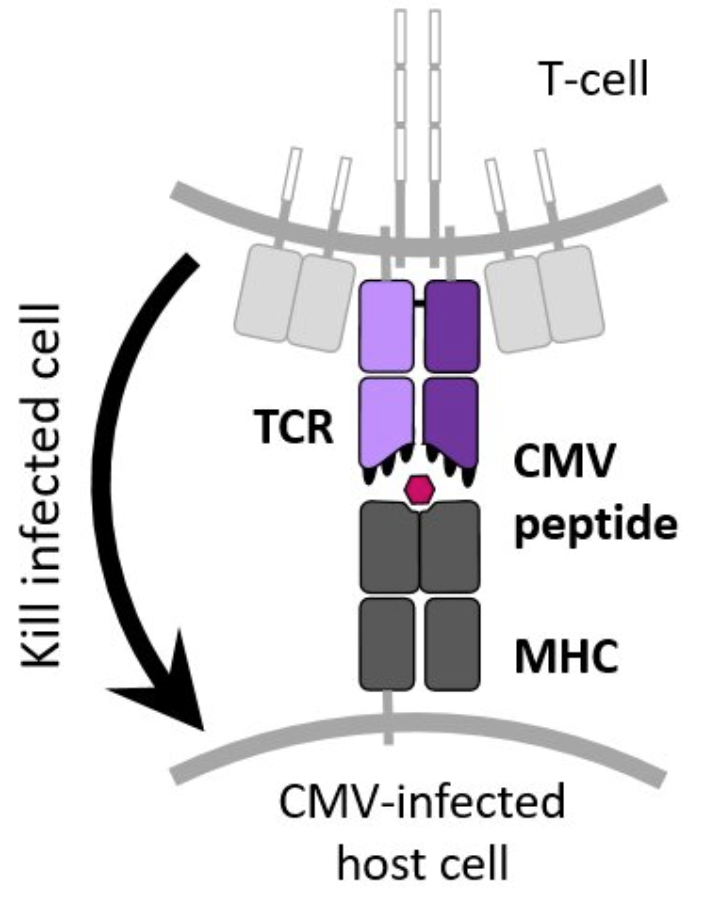
\includegraphics[width=0.6\linewidth]{Figures/TCR.png}
\\
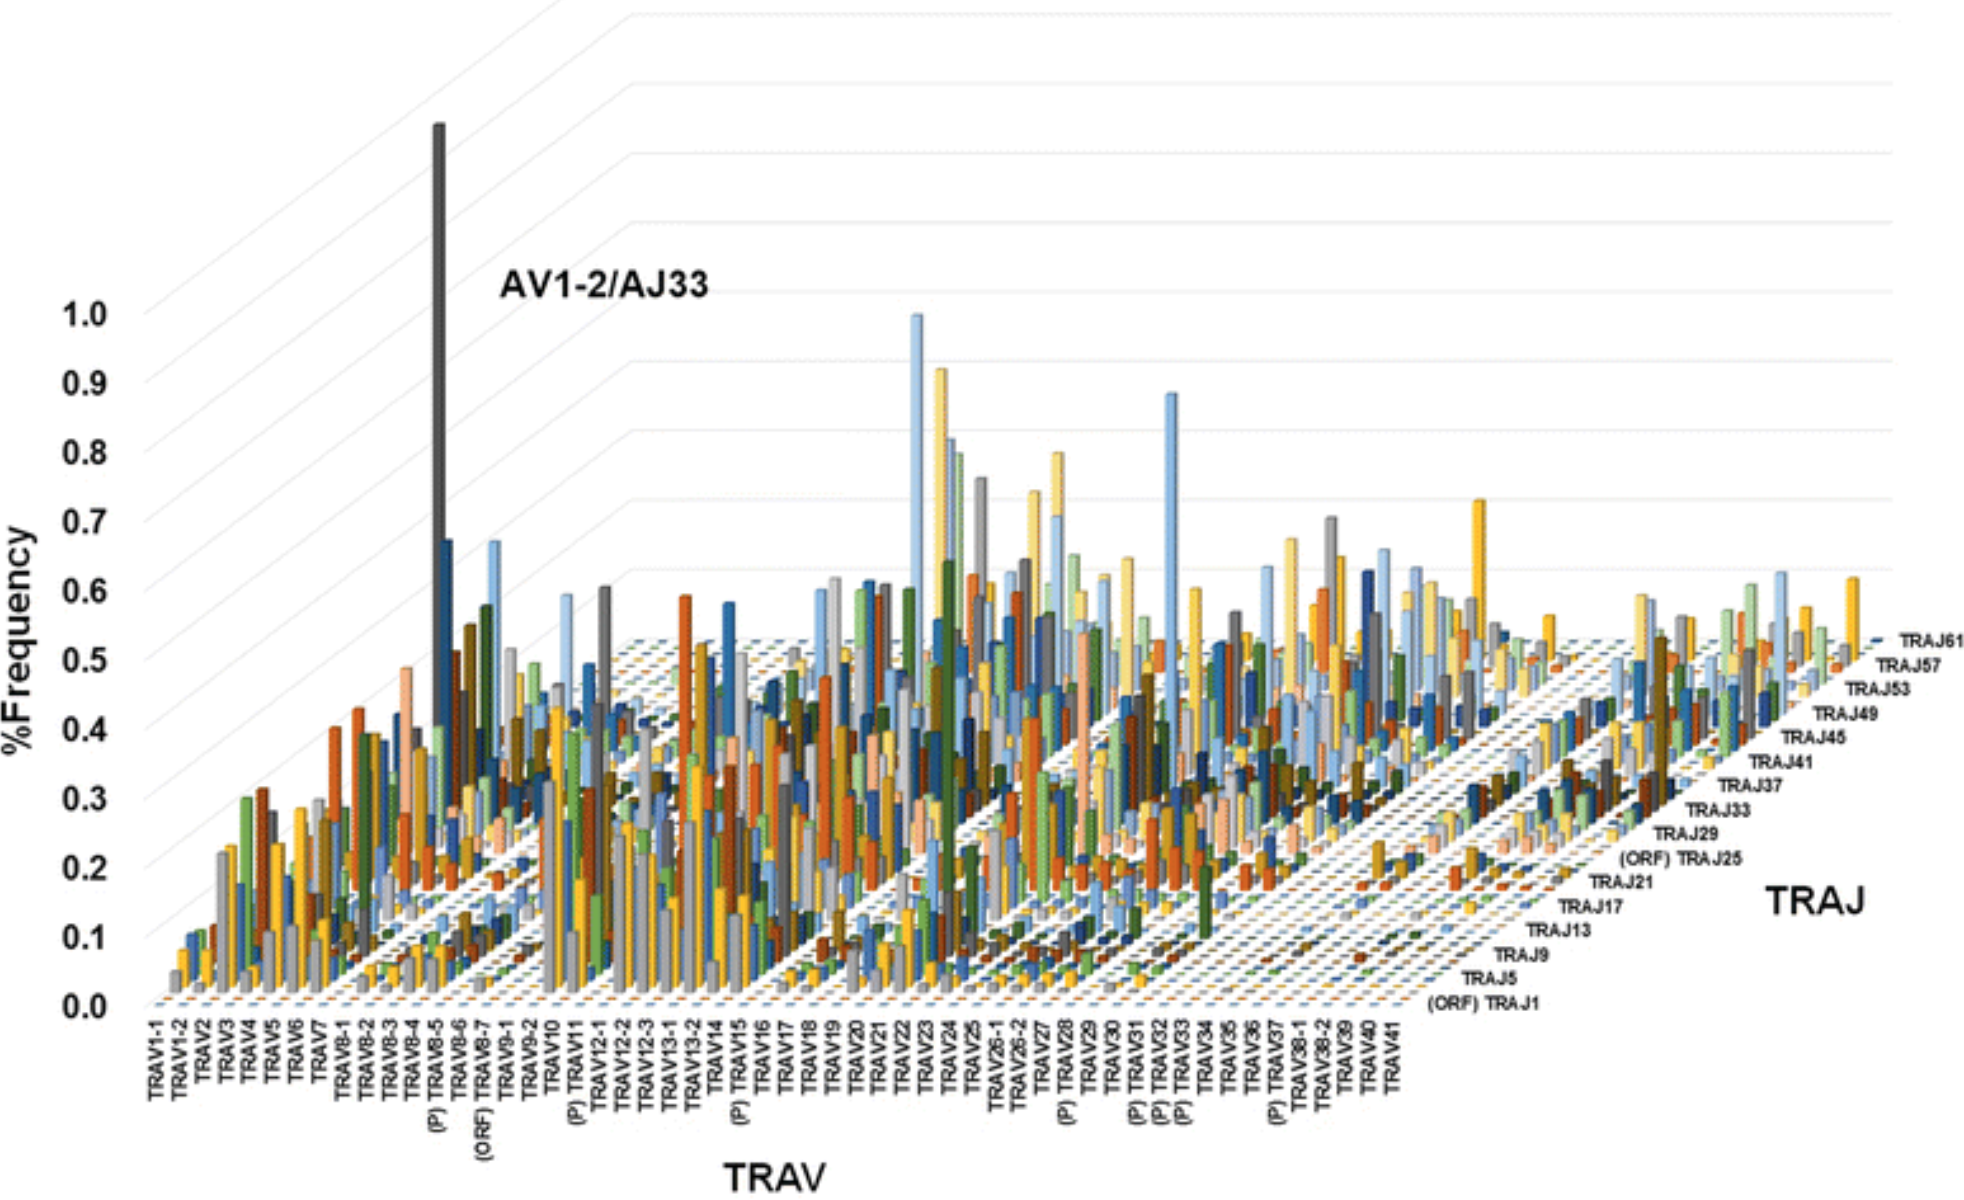
\includegraphics[width=0.8\linewidth]{Figures/TCRRepertoire.png}
\end{center}
\end{minipage}
\end{frame}

\begin{frame}\frametitle{TCR Distributions}
\begin{center}
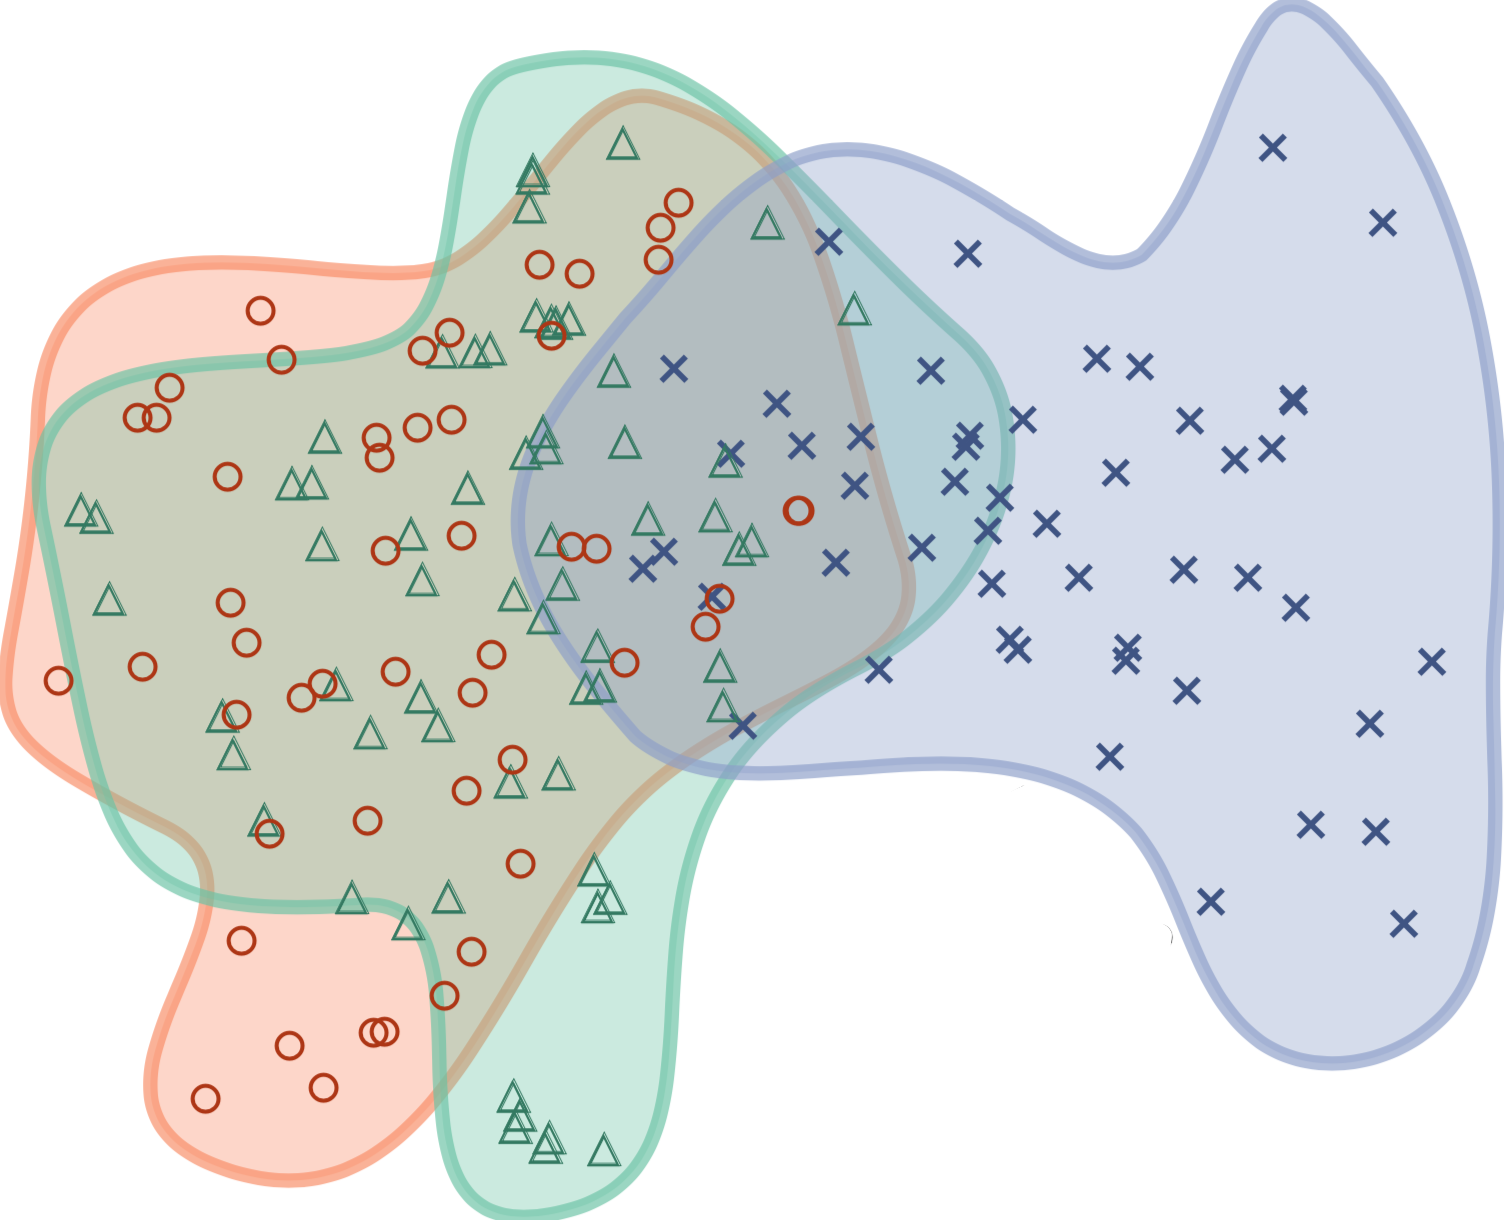
\includegraphics[width=0.8\linewidth]{Figures/TCRDistributions.png}
\end{center}
\end{frame}

\begin{frame}\frametitle{TCR Distributions}
\begin{center}
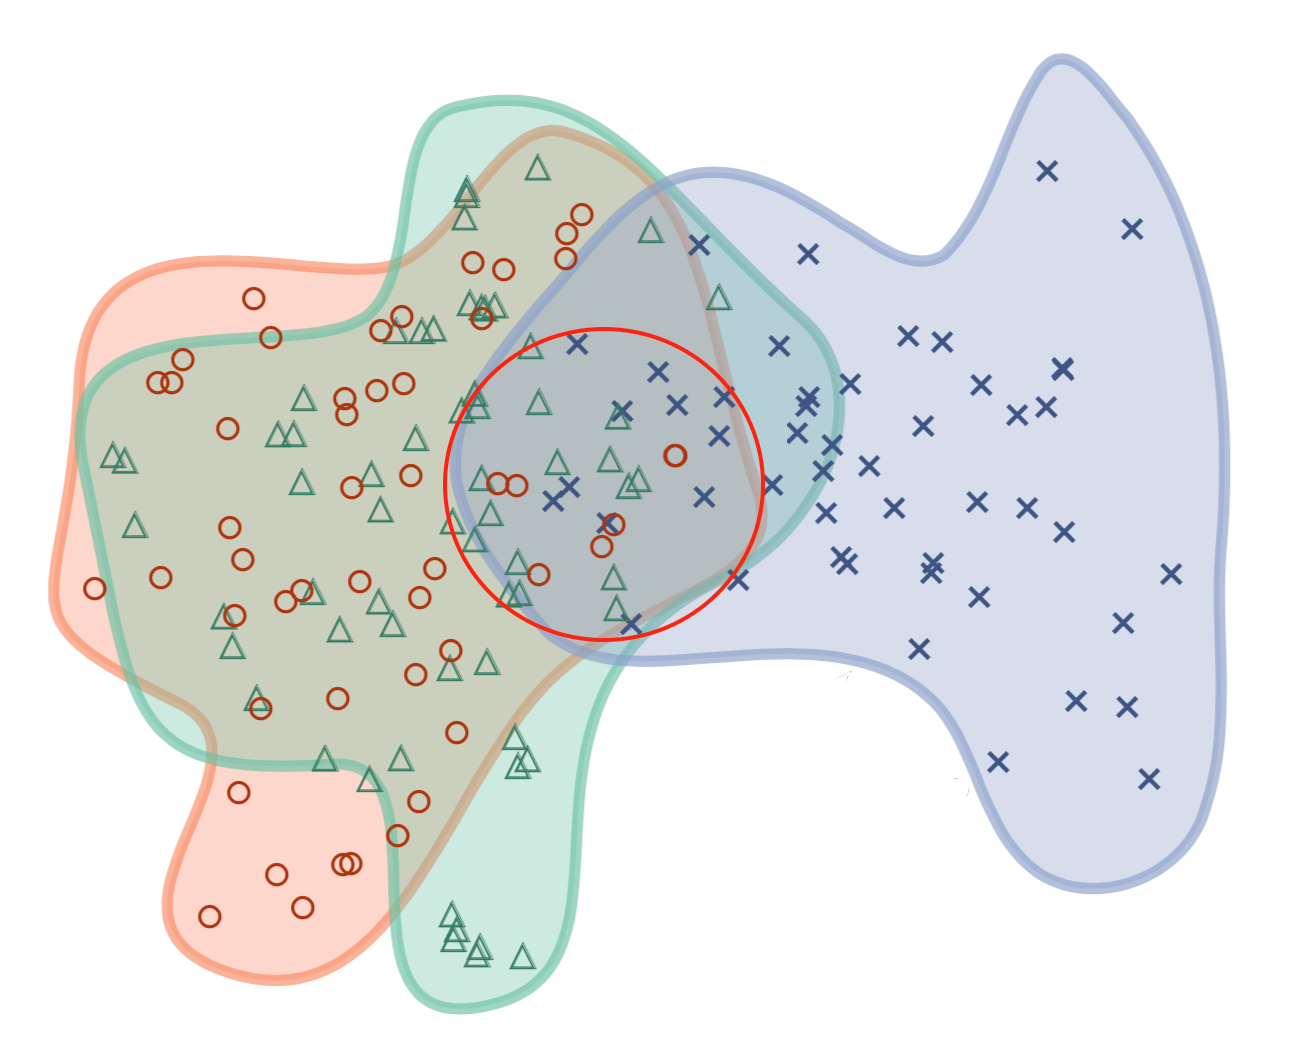
\includegraphics[width=0.8\linewidth]{Figures/TCR_shared.png}
\\
These TCRs seem interesting...
\end{center}
\end{frame}

\begin{frame}\frametitle{TCR Distributions}
\begin{center}
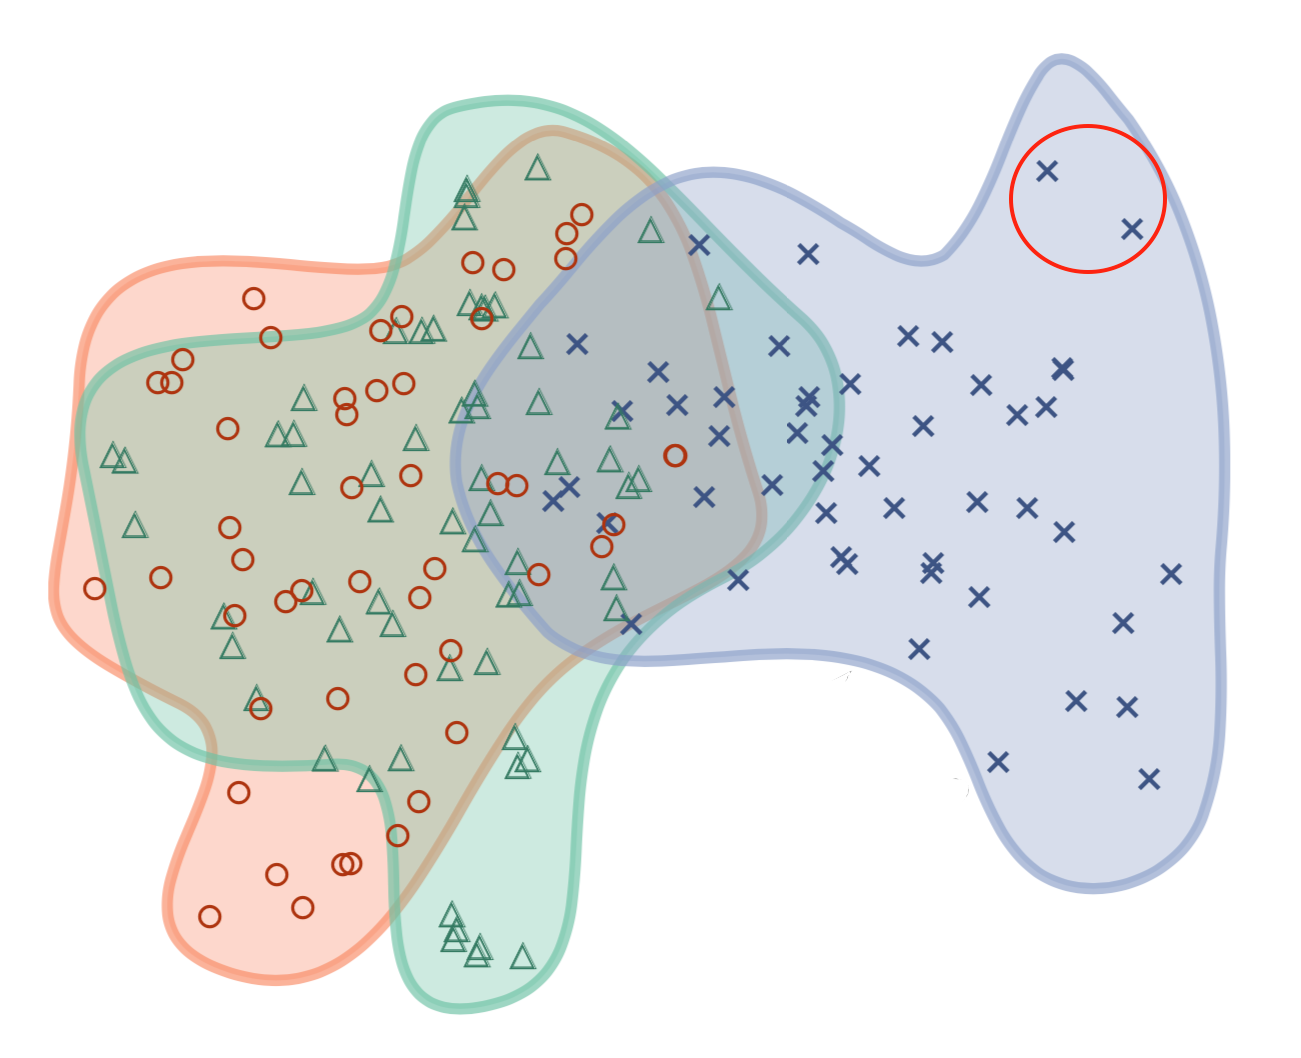
\includegraphics[width=0.8\linewidth]{Figures/TCR_far.png}
\\
These ones also seem interesting...
\end{center}
\end{frame}

\begin{frame}\frametitle{Scientific questions}
It would be nice to have a rigorous method of answering questions like...
\bigskip
\begin{itemize}
\item How different is a repertoire of a vaccinated donor from a repertoire of an unvaccinated donor?
\bigskip
\item Which regions of TCR sequence space are significantly different between donors? 
\bigskip
\item
Which TCRs comprise the largest discrepancies between donors?
\end{itemize}
\end{frame}

\begin{frame}\frametitle{Why is this difficult?}
\begin{itemize}
\item
Comparing discrete distributions is easy! \\ ...but requires dense sampling
\bigskip
\item
Typical divergences (e.g. Jenson Shannon, $\ell_1$) can't account for unobserved repertoire (dis)similarities
\item[]
\ba
\text{Divergence}
	\left(\begin{pmatrix} \color{Purple} V_1 \\ \color{Fuchsia} V_1 \\ \color{Fuchsia} V_1 \\ \color{ProcessBlue} V_2 \\ \color{ProcessBlue} V_2 \\ \color{LimeGreen} V_3 \end{pmatrix},
		  \begin{pmatrix} \color{Fuchsia} V_1 \\ \color{LimeGreen} V_3 \\ \color{LimeGreen} V_3 \\ \color{LimeGreen} V_3 \\ \color{LimeGreen} V_3 \\ \color{orange} V_4 \end{pmatrix}
	\right)
	& = \color{Fuchsia}{|3 - 1|} \color{black}{+} \color{ProcessBlue}{|2 - 0|} \color{black}{+} \color{LimeGreen}{|1 - 4|} \color{black}{+} \color{orange}{|0 - 1|} \\
	& = 8
\ea
\end{itemize}
\end{frame}

\begin{frame}\frametitle{Extreme sparsity}
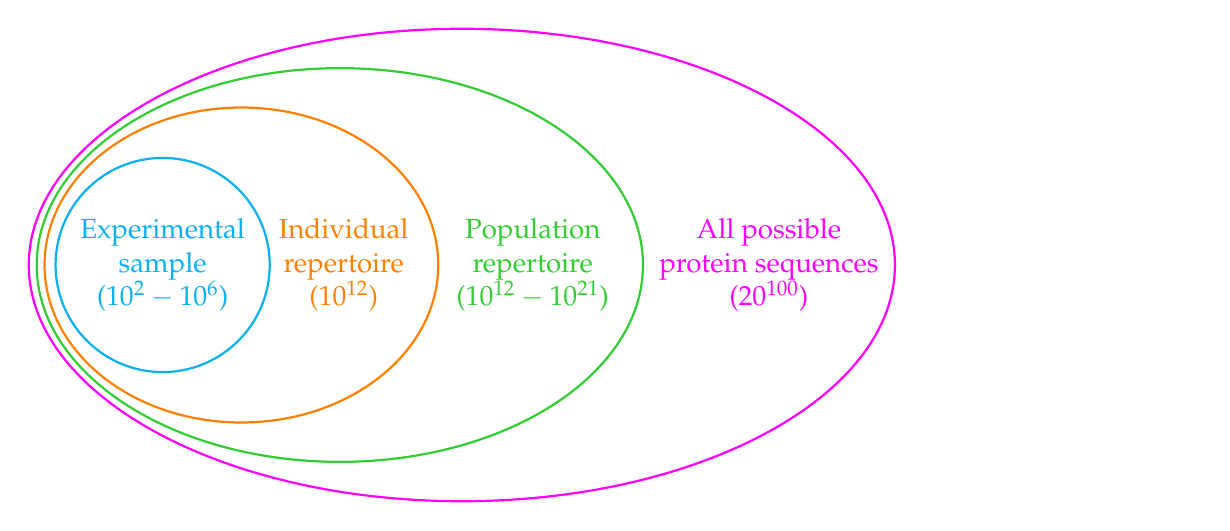
\begin{tikzpicture}
        \node [draw, circle, thick, ProcessBlue, minimum size=2cm, align=center] at   (0,0)   {Experimental\\sample\\($10^2 - 10^6$)};
        \node [draw, ellipse, thick, orange, minimum width=5cm, minimum height=4cm, align=center] at   (1,0) {};
        \node [minimum width=7cm, orange, minimum height=5cm, xshift=3mm, align=center] at   (2,0) {Individual\\repertoire\\($10^{12}$)};
        \node [draw, ellipse, thick, LimeGreen, minimum width=7.7cm, minimum height=5cm, align=center] at (2.25, 0) {};
        \node [minimum width=7cm, LimeGreen, minimum height=5cm, xshift=2.9cm, align=center] at (1.8, 0) {Population\\repertoire\\($10^{12} - 10^{21}$)};
         \node [draw, ellipse, thick, Fuchsia, minimum width=11cm, minimum height=6cm, align=center] at (3.8, 0) {};
         \node [Fuchsia, minimum width=11cm, minimum height=6cm, align=center, xshift=3.9cm] at (3.8, 0) {All possible \\protein sequences \\($20^{100}$)};
    \end{tikzpicture}


\end{frame}

\begin{frame}{What's been done?}
\begin{itemize}
\item[]
Current methods of TCR repertoire comparison:
\bigskip
\begin{itemize}
\item
Gene usage ($+$ CDR3 length)
\begin{itemize}
\medskip
\item \alert{Cons}: see above. Also, CDR3 sequences matter
\end{itemize}
\bigskip
\item
$k$mer comparison
\begin{itemize}
\medskip
\item \alert{Cons}: still high-dimensional, loses positional information
\end{itemize}
\bigskip
\item
$t$-distributed stochastic neighbor embedding (t-SNE)
\begin{itemize}
\medskip
\item \alert{Cons}: high loss of information, questionable immunological meaning
\end{itemize}
\bigskip
\item
\texttt{sumrep}
\begin{itemize}
\medskip
\item \alert{Cons}: descriptive, not inferential
\end{itemize}
\end{itemize}
\end{itemize}
\end{frame}

\section{Optimal transport}

\begin{frame}\frametitle{Problem: Moving dirt}
Consider a pile of dirt and a hole in the ground, with unit volume
\bigskip
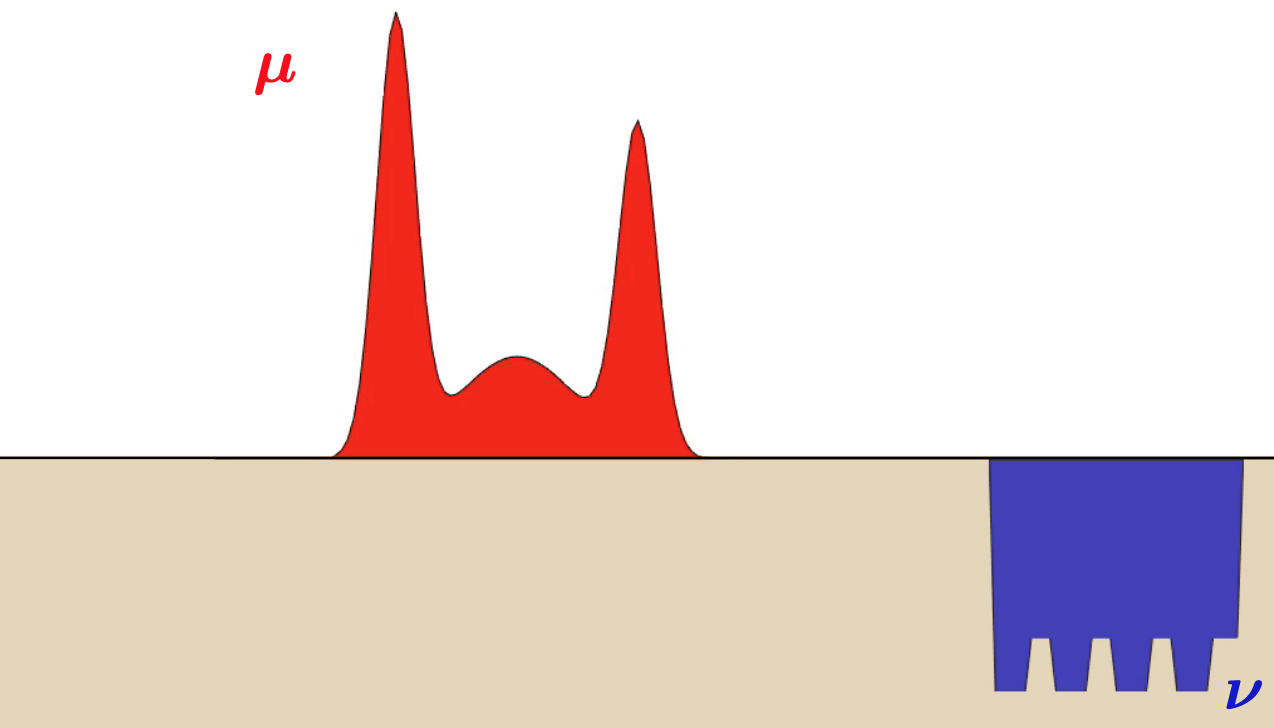
\includegraphics[width=\linewidth]{Figures/EMD_setup.png}
\end{frame}

\begin{frame}\frametitle{Problem: Moving dirt}
How can we fill up the hole using the smallest amount of "effort"?
\bigskip
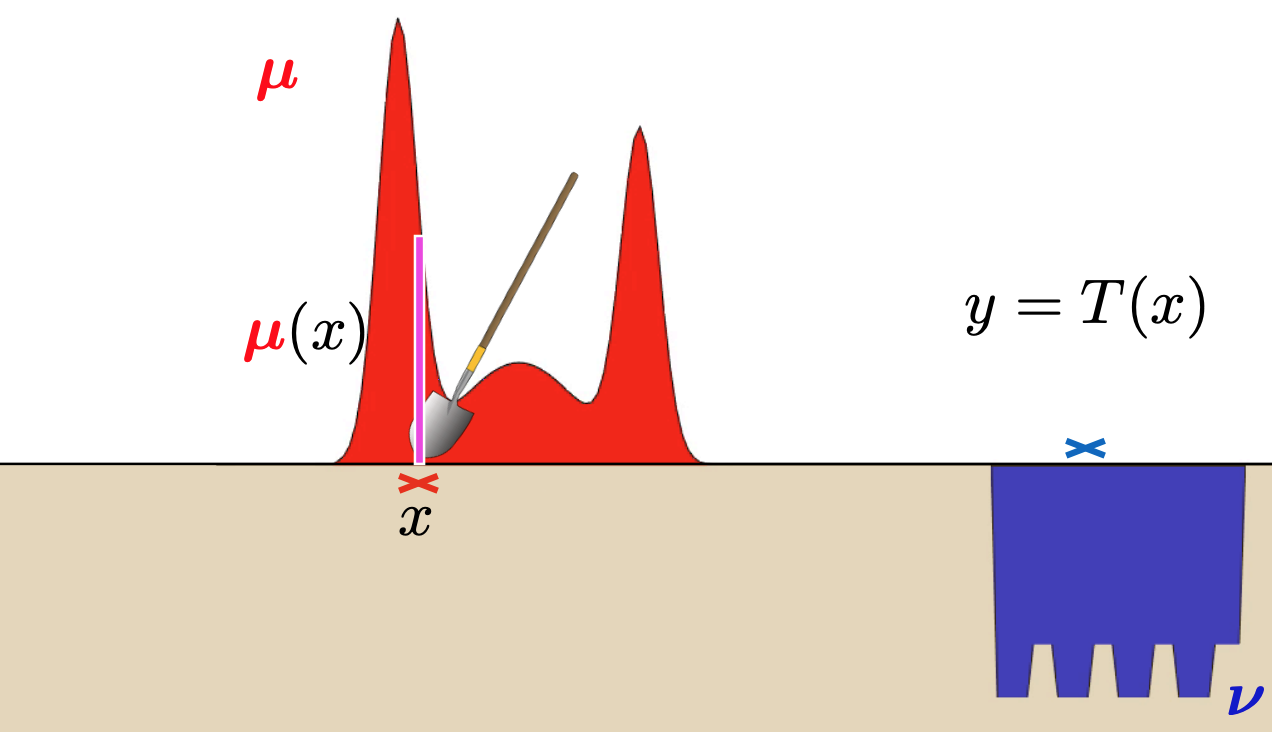
\includegraphics[width=\linewidth]{Figures/EMD_shovel.png}
\end{frame}

\begin{frame}\frametitle{Problem: Dispatching soldiers}
Suppose we need to dispatch some groups of soldiers to some set of stations 
\begin{center}
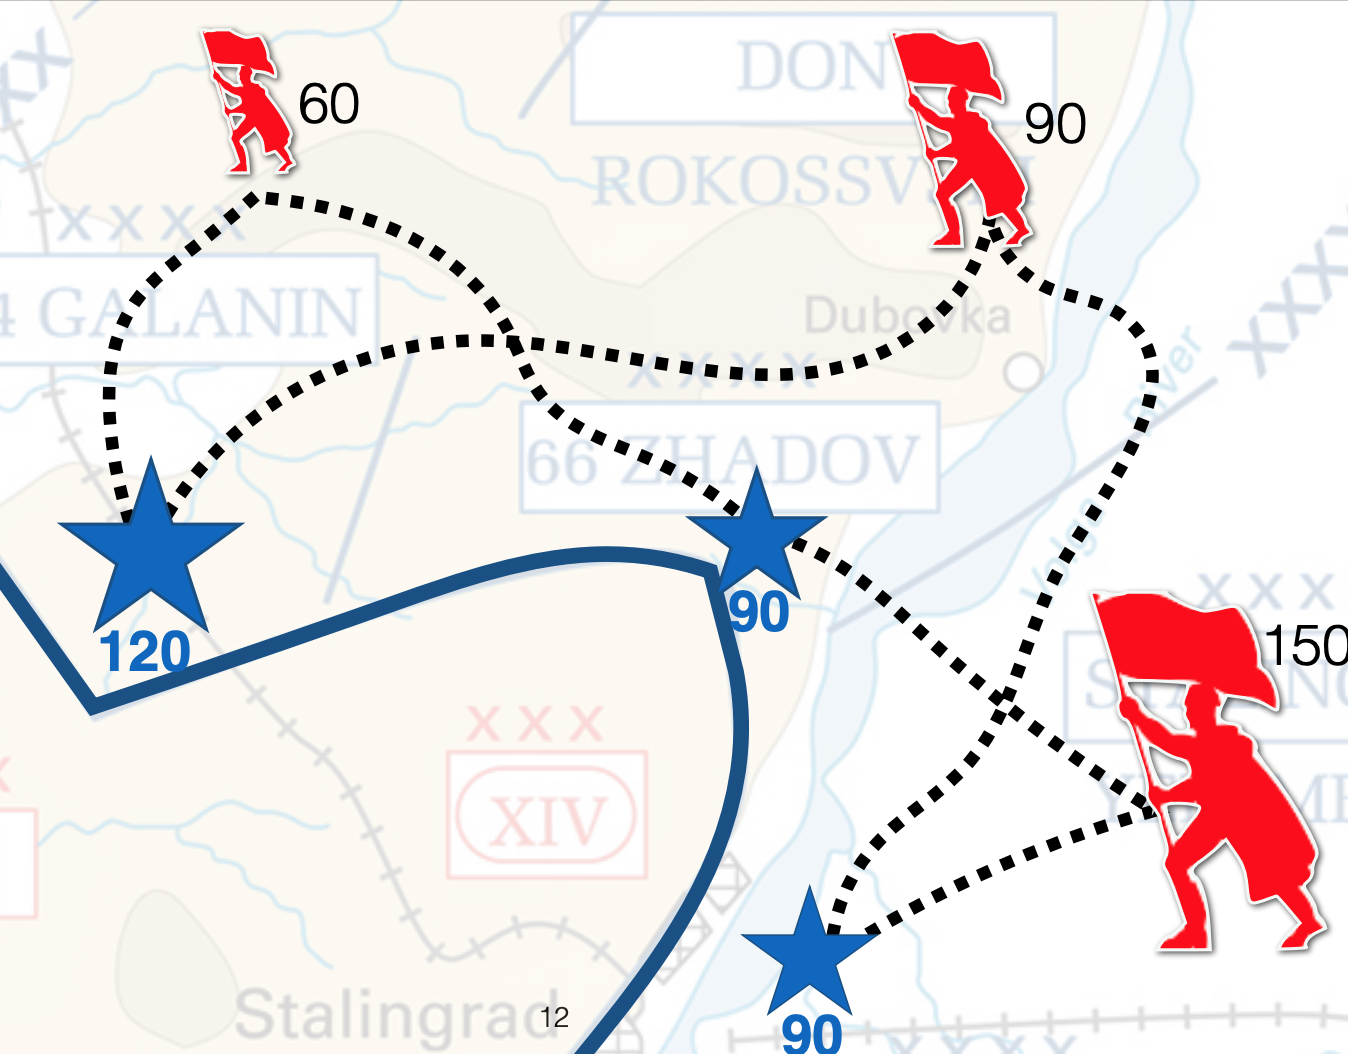
\includegraphics[width=0.8\linewidth]{Figures/soldiers.png}
\end{center}
\end{frame}

\begin{frame}\frametitle{Problem: Dispatching soldiers}
What's the best way to do so to minimize the cumulative distance travelled? 
\begin{center}
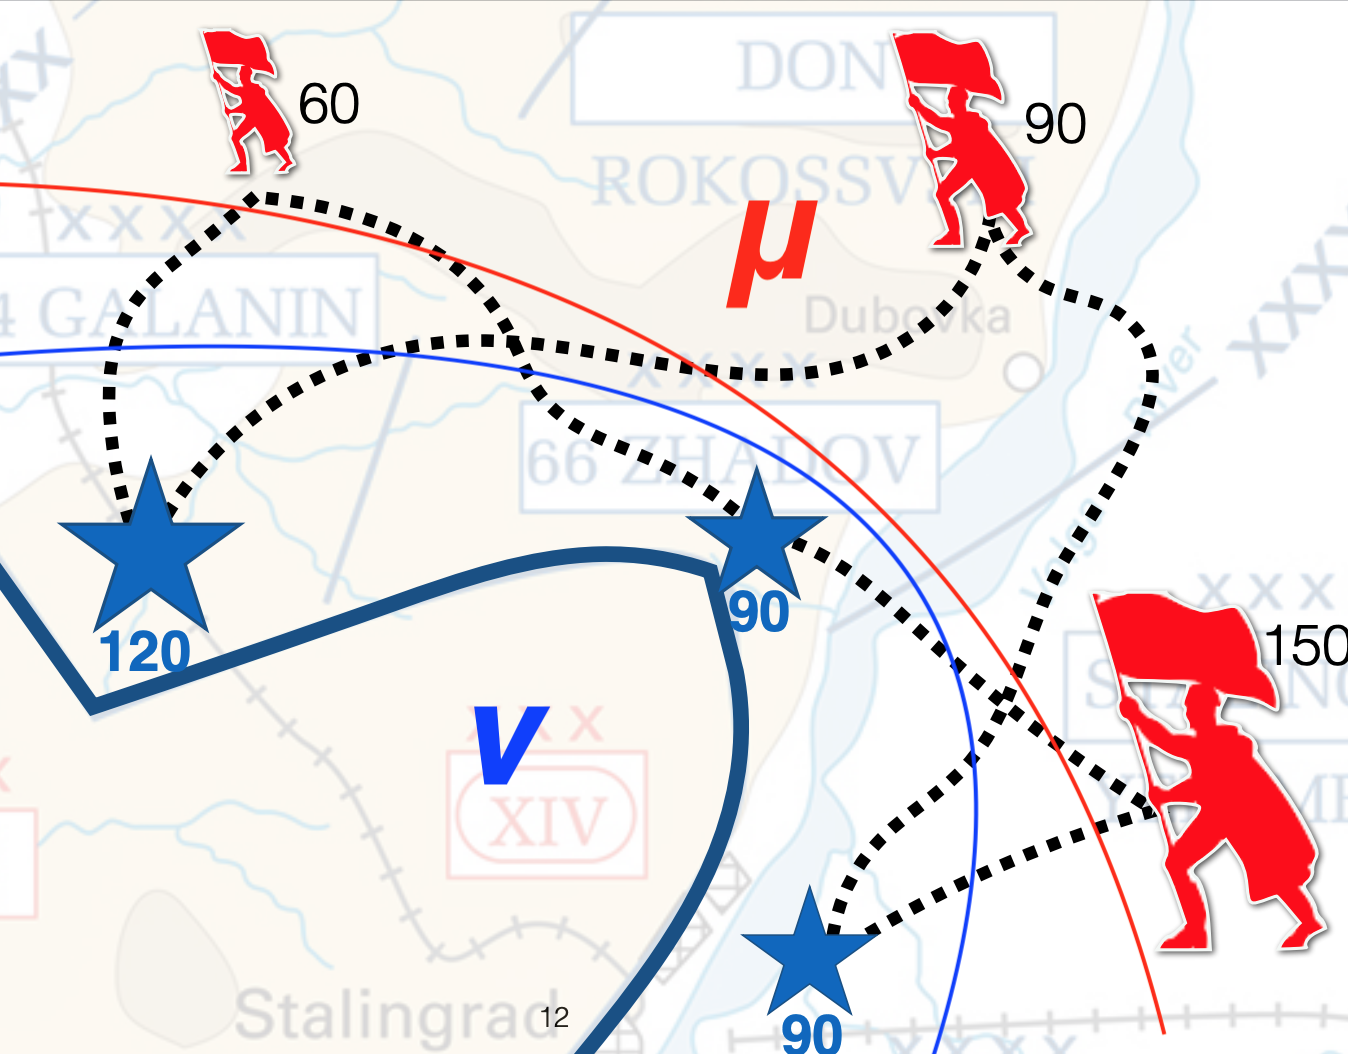
\includegraphics[width=0.8\linewidth]{Figures/soldiers_measures.png}
\end{center}
\end{frame}

\begin{frame}\frametitle{Optimal transport}
\begin{itemize}
\item
The field of optimal transport solves these types of problems
\bigskip
\item
Just need a {\color{Green} distance} ($\equiv$ cost) function 
${\color{Green} d}:\mathcal{X} \times \mathcal{Y} \to \reals^+$ for {\color{Purple} moving} objects around
\bigskip
\item
Optimizations of the form
\begin{align}
	\ & \min_{{\color{violet} \pi} \in \Pi({\color{red} \mu}, {\color{blue} \nu})} 
		\int_{\mathcal X \times \mathcal Y} 
		{\color{Green} d}(x, y) \der {\color{violet} \pi}(x, y) \\
	\equiv & \min_{{\color{violet} \pi} \in 
		\Pi({\color{red} \mu}, {\color{blue} \nu})}
		 \Esub{(X, Y) \sim {\color{violet} \pi}}{ {\color{Green} d}(X, Y) } \\
	\equiv & \mathcal L_{{\color{Green} d}}(
		{\color{red} \mu}, {\color{blue} \nu}) \end{align}
\end{itemize}
\end{frame}

\begin{frame}\frametitle{Wasserstein distance}
\begin{itemize}
\item[]
$
\mathcal L_{{\color{Green} d}}(
		{\color{red} \mu}, {\color{blue} \nu}) 
	\equiv \text{Wasserstein distance between ${\color{red} \mu}$ and ${\color{blue} \nu}$ w.r.t. ${\color{Green} d}$}
$
\bigskip
\item[]
Discrete case:
\ba
\mathcal L_{{\color{Green} \mathbf D}}(
		{\color{red} \mu}, {\color{blue} \nu})
	& = \min_{{\color{Purple} \mathbf P} \in \Pi({\color{red} \mu}, {\color{blue} \nu})}
		\sum_{i=1}^n \sum_{j=1}^m \mathbf {\color{Green} D}_{i,j} \mathbf {\color{Purple} \mathbf P}_{i,j}
\ea
where
$\mathbf {\color{Green} D}_{i,j} = {\color{Green} d}(x_i, y_j)$ 
and
$\mathbf {\color{Purple} \mathbf P}_{i,j} = {\color{violet} \pi}(x_i, y_j)$
\end{itemize}
\end{frame}

\begin{frame}\frametitle{Admissible couplings}
\begin{itemize}
\item
Write discrete distributions ${\color{red} \mu}, {\color{blue} \nu}$ as vectors ${\color{red} \mathbf r}, {\color{blue} \mathbf c}$ respectively.
\bigskip
\item
Set of admissible couplings:
\ba
\Pi({\color{red} \mathbf r}, {\color{blue} \mathbf c}) 
	= \set{ {\color{Purple} \mathbf P} \in \reals_+^{n \times m} : 
	\mathbf {\color{Purple} \mathbf P} \mathbf{1}_m = {\color{red} \mathbf r} \text{ and }
	\mathbf {\color{Purple} \mathbf P}^\mathsf{T} \mathbf{1}_n = {\color{blue} \mathbf c} }
\ea
\item Then
\begin{align}
\mathcal L_{{\color{Green} \mathbf D}}(
		{\color{red} \mathbf r}, {\color{blue} \mathbf c})
	& = \min_{{\color{Purple} \mathbf P} \in \Pi({\color{red} \mathbf r} , {\color{blue} \mathbf c})}
		\sum_{i=1}^n \sum_{j=1}^m \mathbf {\color{Green} D}_{i,j} \mathbf {\color{Purple} \mathbf P}_{i,j} \\
	& = \min_{{\color{Purple} \mathbf P} \in \Pi({\color{red} \mathbf r} , {\color{blue} \mathbf c})} 
		\langle \mathbf {\color{Green} D}, {\color{Purple} \mathbf P} \rangle 
\end{align}
is a linear program over a convex polytope
\medskip
\item
Complexity: $\mathcal O(k^3 \log k)$, $k = \max(n, m)$  \Sadey
\end{itemize}
\end{frame}

\begin{frame}\frametitle{Sinkhorn distance}
\begin{itemize}
\item
Cuturi (2013): let's regularize for high entropy of the couplings ${\color{Purple} \mathbf P}$ for simplicity
\bigskip
\item
In particular, they introduce the Sinkhorn distance 
\begin{align}
\mathcal L_{{\color{Green} \mathbf D}}^\lambda(
		{\color{red} \mathbf r}, {\color{blue} \mathbf c})
	:= \left\langle {\color{Green} \mathbf D}, {\color{Purple} \mathbf P}_{{\color{red} \mathbf r}, {\color{blue} \mathbf c}}^\lambda \right\rangle
\end{align}
where
\begin{align}
{\color{Purple} \mathbf P}_{{\color{red} \mathbf r}, {\color{blue} \mathbf c}}^\lambda 
= \argmin_{{\color{Purple} \mathbf P} \in \Pi({\color{red} \mathbf r} , {\color{blue} \mathbf c})}
	\left\{ \langle {\color{Green} \mathbf D}, {\color{Purple} \mathbf P} \rangle - \frac{1}{\lambda} h({\color{Purple} \mathbf P}) \right\}
\end{align}
and $h({\color{Purple} \mathbf P}) 
	:= - \sum_{i=1}^d \sum_{j=1}^d {\color{Purple} \mathbf P}_{i,j} \log({\color{Purple} \mathbf P}_{i,j})$ is the Shannon entropy of ${\color{Purple} \mathbf P}$.
\end{itemize}
\end{frame}

\begin{frame}\frametitle{What is Sinkhorn doing?}
\begin{itemize}
\item
Turns out we're constraining region to a new region $\Pi_\alpha$ with
\begin{align}
\Pi_\alpha({\color{red} \mathbf r} , {\color{blue} \mathbf c})
	= \left\{ {\color{Purple} \mathbf P} \in \Pi({\color{red} \mathbf r} , {\color{blue} \mathbf c}) : 
		\text{KL}\left({\color{Purple} \mathbf P} \ \big{|}\big| \ {\color{red} \mathbf r} {\color{blue} \mathbf c}^{\mathsf T} \right) \le \alpha \right\}.
\end{align}
so that
\ba
\mathcal L_{{\color{Green} \mathbf D}}^\lambda(
		{\color{red} \mathbf r}, {\color{blue} \mathbf c})
	= \min_{{\color{Purple} \mathbf P} \in \Pi_\alpha({\color{red} \mathbf r} , {\color{blue} \mathbf c})} 
		\langle \mathbf {\color{Green} D}, {\color{Purple} \mathbf P} \rangle 
\ea
\begin{center}
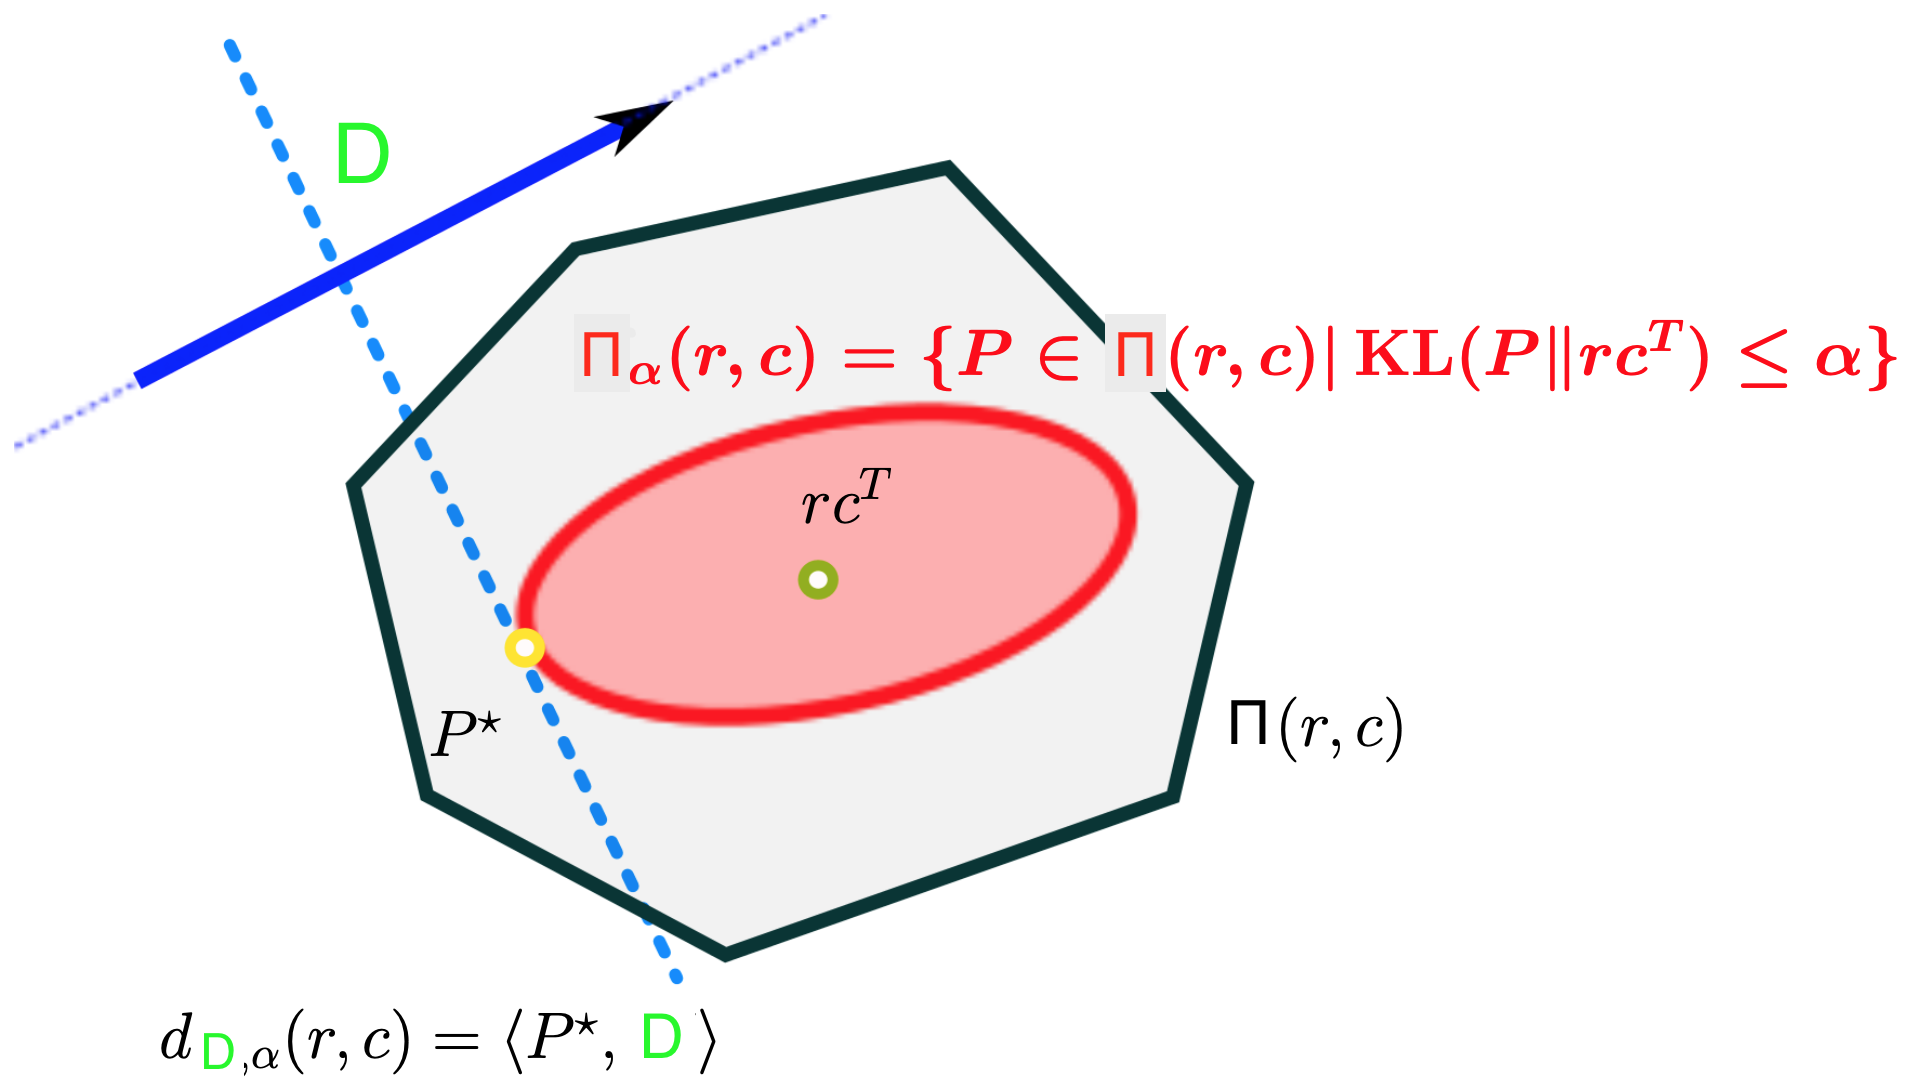
\includegraphics[width=0.7\linewidth]{Figures/Polytope.png}
\end{center}

\end{itemize}

\end{frame}

\section{Toy example}

\begin{frame}\frametitle{Example: discrete distribution}
\begin{itemize}
\item[]
Let $\mathcal X = \{{\color{orange} 1}, {\color{orange} 2}, {\color{orange} 4}\}$, 
$\mathcal Y = \{ {\color{ProcessBlue} 1}, {\color{ProcessBlue} 3}, {\color{ProcessBlue} 5}\}$ and define distributions $\color{red}\mu$ and $\color{blue}\nu$ via
\ba
{\color{red} \mu} ({\color{orange} 1}) & = 0.6, 
\ {\color{red} \mu} ({\color{orange} 2}) = 0.3, 
\ {\color{red} \mu} ({\color{orange} 4}) = 0.1 \\
{\color{blue} \nu} ({\color{ProcessBlue} 1}) & = 0.3, 
\ {\color{blue} \nu}({\color{ProcessBlue} 3}) = 0.5, 
\ {\color{blue} \nu}({\color{ProcessBlue} 5}) = 0.2.
\ea
\vspace{-2em}
\begin{center}
\includegraphics[width=0.8\linewidth]{/Users/brandenolson/Code/Matsen/Manuscripts/transport/pmf.png}
\end{center}
\end{itemize}
\end{frame}

\begin{frame}\frametitle{Example: discrete distribution}
\begin{itemize}
\item[]
The cost matrix ${\color{Green} \mathbf D}_{{\color{orange} i}{\color{ProcessBlue} j}} = {\color{Green} d}({\color{orange} x_i}, {\color{ProcessBlue} y_j})$, using 
${\color{Green} d}({\color{orange} x}, {\color{ProcessBlue} y}) = |{\color{orange} x} - {\color{ProcessBlue} y}|$ as our metric, is
\ba
{\color{Green} \mathbf D} = 
	\begin{blockarray}{cccc}
	& {\color{ProcessBlue} 1} & {\color{ProcessBlue} 3} & {\color{ProcessBlue} 5} \\
	\begin{block}{c(ccc)}
		{\color{orange} 1} & |{\color{orange} 1} - {\color{ProcessBlue} 1}| & |{\color{orange} 1} - {\color{ProcessBlue} 3}| & |{\color{orange} 1} - {\color{ProcessBlue} 5}| \\
		{\color{orange} 2} & |{\color{orange} 2} - {\color{ProcessBlue} 1}| & |{\color{orange} 2} - {\color{ProcessBlue} 3}| & |{\color{orange} 2} - {\color{ProcessBlue} 5}| \\
		{\color{orange} 4} & |{\color{orange} 4} - {\color{ProcessBlue} 1}| & |{\color{orange} 4} - {\color{ProcessBlue} 3}| & |{\color{orange} 4} - {\color{ProcessBlue} 5}| \\
	\end{block}
\end{blockarray}
=
\begin{blockarray}{cccc}
	& {\color{ProcessBlue} 1} & {\color{ProcessBlue} 3} & {\color{ProcessBlue} 5} \\
	\begin{block}{c(ccc)}
		{\color{orange} 1} & \color{Green}0 & \color{Green}2 & \color{Green}4 \\
		{\color{orange} 2} & \color{Green}1 & \color{Green}1 & \color{Green}3 \\
		{\color{orange} 4} & \color{Green}3 & \color{Green}1 & \color{Green}1 \\
	\end{block}
\end{blockarray}
\ea
\vspace{-3em}
\begin{center}
\includegraphics[width=0.7\linewidth]{/Users/brandenolson/Code/Matsen/Manuscripts/transport/pmf.png}
\end{center}
\end{itemize}
\end{frame}

\begin{frame}\frametitle{Example: "proof" by inspection}
\begin{minipage}{0.49\linewidth}
\begin{itemize}
\item
${\color{blue} \nu}$ needs 0.2 mass at $x = 5$;  the closest mass from ${\color{red} \mu}$ is 0.1 unit at $x = 4$
\item
${\color{blue} \nu}$ still needs 0.1 unit of mass for $x = 5$; get from ${\color{red} \mu}$ at next closest value, $x = 2$
\item
This leaves 0.2 units from ${\color{red} \mu}$ at $x = 2$ which can be moved to $x = 3$ for ${\color{blue} \nu}$
\item
Remaining 0.3 units needed at $x = 3$ for ${\color{blue} \nu}$ can be obtained from $x = 1$ in ${\color{red} \mu}$
\item
This leaves 0.3 units at $x = 1$ for ${\color{blue} \nu}$, as desired.
\end{itemize}
\end{minipage}
\begin{minipage}{0.49\linewidth}
\includegraphics[width=\linewidth]{/Users/brandenolson/Code/Matsen/Manuscripts/transport/pmf.png}
\footnotesize
\vspace{-1em}
\ba
{\color{Purple} \mathbf P^*} & = \begin{blockarray}{cccc}
	& {\color{ProcessBlue} 1} & {\color{ProcessBlue} 3} & {\color{ProcessBlue} 5} \\
	\begin{block}{c(ccc)}
		{\color{orange} 1} & \color{Purple} 0.3 & \color{Purple} 0.3 & \color{Purple} 0 \\
		{\color{orange} 2} & \color{Purple} 0 & \color{Purple}  0.2 & \color{Purple} 0.1 \\
		{\color{orange} 4} & \color{Purple} 0 & \color{Purple} 0 & \color{Purple} 0.1 \\
	\end{block}
\end{blockarray} \\
\mathcal L_{{\color{Green} \mathbf D}}(\color{red}\mu, \color{blue}\nu) 
	& = \langle \mathbf {\color{Green} D}, {\color{Purple} \mathbf P^*} \rangle \\
	& = {\color{Green} 2} \cdot {\color{Purple} 0.3} + {\color{Green} 1} \cdot {\color{Purple} 0.2} + {\color{Green} 3} \cdot {\color{Purple} 0.1} + {\color{Green} 1} \cdot {\color{Purple} 0.1} \\
	& = 1.2
\ea
\end{minipage}
\end{frame}

\begin{frame}[fragile]\frametitle{Example: rigorous solution}
\small
To solve for ${\color{Purple} \mathbf P^*}$ rigorously, we can set up a linear program using the row-sums and column-sums constraints:
\bigskip
\ba
\;& \text{minimize} \ {\color{Purple} \mathbf P}_{1,2} + 4{\color{Purple} \mathbf P}_{1,3} + {\color{Purple} \mathbf P}_{2,1} +  {\color{Purple} \mathbf P}_{2, 2} + 3{\color{Purple} \mathbf P}_{2,3} + 3{\color{Purple} \mathbf P}_{3,1} + {\color{Purple} \mathbf P}_{3,2} + {\color{Purple} \mathbf P}_{3, 3} \\
& \text{subject to} \begin{cases}
	 {\color{Purple} \mathbf P}_{1,1} + {\color{Purple} \mathbf P}_{1,2} + {\color{Purple} \mathbf P}_{1,3} = 0.6 \\
	 {\color{Purple} \mathbf P}_{2,1} + {\color{Purple} \mathbf P}_{2,2} + {\color{Purple} \mathbf P}_{2,3} = 0.3 \\
	 {\color{Purple} \mathbf P}_{3,1} + {\color{Purple} \mathbf P}_{3,2} + {\color{Purple} \mathbf P}_{3,3} = 0.1 \\
	 {\color{Purple} \mathbf P}_{1,1} + {\color{Purple} \mathbf P}_{2,1} + {\color{Purple} \mathbf P}_{3,1} = 0.3 \\
	 {\color{Purple} \mathbf P}_{1,2} + {\color{Purple} \mathbf P}_{2,2} + {\color{Purple} \mathbf P}_{3,2} = 0.5 \\
	 {\color{Purple} \mathbf P}_{1,3} + {\color{Purple} \mathbf P}_{2,3} + {\color{Purple} \mathbf P}_{3,3} = 0.2 \\
	 0 \le {\color{Purple} \mathbf P}_{i,j} \le 1 \ \forall i,j 
\end{cases}
\ea
\end{frame}

\begin{frame}[fragile]\frametitle{Example: rigorous solution}
Using the numerical solver \texttt{lpSolve::lp} in R, we verify the above:
\bigskip
\begin{lstlisting}
> lp_sol                      
Success: the objective function is 1.2                   
> lp_sol$solution %>% matrix(byrow=T, nrow=3)               
     [,1] [,2] [,3]           
[1,]  0.3  0.3  0.0           
[2,]  0.0  0.2  0.1           
[3,]  0.0  0.0  0.1 
\end{lstlisting}
\end{frame}

\begin{frame}\frametitle{Example: Sinkhorn solution}
Using \texttt{pot}, a Python solver for the Sinkhorn distance:
\begin{center}
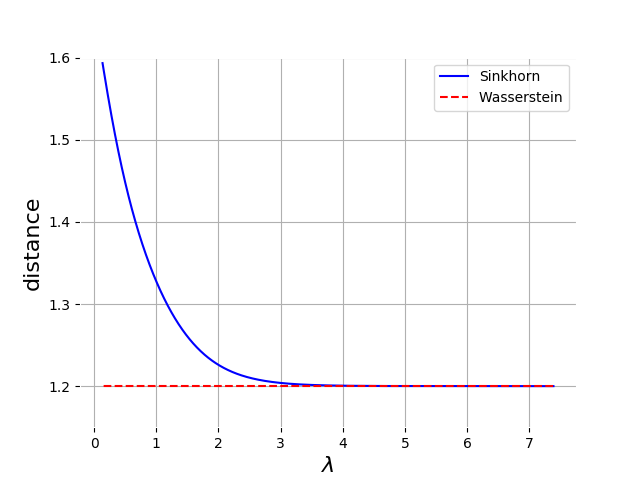
\includegraphics[width=0.8\linewidth]{Figures/lambda.png}
\end{center}
\end{frame}

\begin{frame}\frametitle{Example: Sinkhorn solution}
\begin{itemize}
\item Transportation matrices:
\begin{align*}
{\color{Purple} \mathbf P}_{{\color{red} \mu}, {\color{blue} \nu}}^{\lambda = 200}
 & = 
\begin{pmatrix} 0.3 & 0.3 & 0 \\
				0 & 0.2 & 0.1 \\
				0 & 0 & 0.1
	\end{pmatrix}
	= {\color{Purple} \mathbf P}_{{\color{red} \mu}, {\color{blue} \nu}}^* \\
{\color{Purple} \mathbf P}_{{\color{red} \mu}, {\color{blue} \nu}}^{\lambda = 1}
 & = 
\begin{pmatrix}
	0.269 & 0.257 & 0.073 \\
    0.029 & 0.210 & 0.059 \\
    0 & 0.032 & 0.067 \\
\end{pmatrix} \\
{\color{Purple} \mathbf P}_{{\color{red} \mu}, {\color{blue} \nu}}^{\lambda = 1/200}
	& = 
\begin{pmatrix}
	0.180 & 0.299 &  0.119 \\
    0.089 & 0.150 & 0.060 \\
    0.029 & 0.050 & 0.020 \\
\end{pmatrix}
\end{align*}
\item
Recover ${\color{Purple} \mathbf P}_{{\color{red} \mu}, {\color{blue} \nu}}^*$ as $\lambda\to\infty$ (in theory) \Smiley
\medskip
\item
High enough $\lambda$ yields \texttt{NaN} in practice \Sadey
\end{itemize}
\end{frame}

\section{Application to TCRs}

\begin{frame}\frametitle{TCR distances}
\begin{minipage}{0.49\linewidth}
\begin{itemize}
\item
We need a distance between TCRs to apply these methods
\bigskip
\item
This is very much a research question, as T cell receptors are intricate proteins constructed from genes of multiple loci
\bigskip
\item
Nonetheless, we have some options
\end{itemize}
\end{minipage}
\begin{minipage}{0.49\linewidth}
\ba
{\color{Green} d} \left(
\
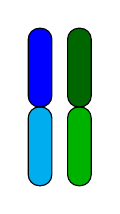
\begin{tikzpicture}[baseline={(1, 1)}]
	\draw[rounded corners, fill=cyan] (0, 0) rectangle (0.3, 1) {};
	\draw[rounded corners, fill=blue] (0, 1) rectangle (0.3, 2) {};
	
		\draw[rounded corners, fill=black!30!green] (0.5, 0) rectangle (0.8, 1) {};
	\draw[rounded corners, fill=black!60!green] (0.5, 1) rectangle (0.8, 2) {};
\end{tikzpicture}
\ , \
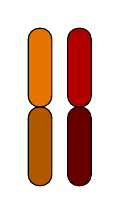
\begin{tikzpicture}[baseline={(1, 1)}]
	\draw[rounded corners, fill=black!30!orange] (0, 0) rectangle (0.3, 1) {};
	\draw[rounded corners, fill=black!10!orange] (0, 1) rectangle (0.3, 2) {};
	
		\draw[rounded corners, fill=black!60!red] (0.5, 0) rectangle (0.8, 1) {};
	\draw[rounded corners, fill=black!30!red] (0.5, 1) rectangle (0.8, 2) {};
\end{tikzpicture}
\
\right)
= ?
\ea

\end{minipage}
\end{frame}

\begin{frame}\frametitle{Option 1: TCRdist [Dash et al. '17]}
\begin{align}
\text{TCRdist}(r_1, r_2)
	& := \sum_{p \in \text{{\color{ProcessBlue} CDR positions}}} 
		\sum_{(a_1, a_2) \in p}
		{\color{Orange} w}(p) 
		\text{{\color{Green} AAdist}}(a_1, a_2; p)
\end{align}

where:
\footnotesize
\begin{itemize}
\item
$\text{{\color{ProcessBlue} CDR positions}} 
	:= \{\text{CDR1}\alpha, \text{CDR2}\alpha, \text{CDR2.5}\alpha, 
		\text{CDR3}\alpha,
		 \text{CDR1}\beta, \text{CDR2}\beta, \text{CDR2.5}\beta, \text{CDR3}\beta\}$
\item 
$ {\color{Orange} w}(p) := \begin{cases} 3, & p \in \{\text{CDR3}\alpha, \text{CDR3}\beta\} \\
						1, & \text{else}
		\end{cases}$
\item
$ \text{{\color{Green} AAdist}}(a_1, a_2; p) := 
\begin{cases}
	0, & a_1 = a_2 \\
	8, & a_1 = \text{`}\texttt{-}\text{'} \oplus a_2 = \text{`}\texttt{-}\text{'}, 
		\ p \in \{\text{CDR3}\alpha, \text{CDR3}\beta\} \\
	4, & a_1 = \text{`}\texttt{-}\text{'} \oplus a_2 = \text{`}\texttt{-}\text{'}, 
		\ p \not\in \{\text{CDR3}\alpha, \text{CDR3}\beta\} \\

	4 - \min(0,  \text{{\color{Purple} BLOSUM62}}(a_1, a_2)), & \text{else} 
\end{cases}$ 
\item
{\color{Purple} BLOSUM62}: widely-used AA substitution matrix
[Henikoff '92]
\end{itemize}
\end{frame}

\begin{frame}
\begin{center}
\includegraphics[width=0.7\linewidth]{Figures/TCRdist.png}
\end{center}
\end{frame}

\begin{frame}\frametitle{Option 2: VAE embeddings}
\begin{itemize}
\item
Another possibility: use a variational autoencoder (VAE)
\bigskip
\item
Let $D_1 = ({\color{red} \bs_{1}^1, \dotsc, \bs_{n}^1})$ and $D_2 = ({\color{blue} \bs_{1}^2, \dotsc, \bs_{m}^2} )$ be TR$\beta$ sequences from donors 1 \& 2
\bigskip
\item
Get latent space embedding coordinates ${\color{red} \bz_1^1, \dotsc, \bz_n^1}$ and ${\color{blue} \bz_1^2, \dotsc, \bz_m^2}$
 where
${\color{Purple} \bz_j^i} = \phi_\theta({\color{Purple} \bs_j^i}) \in \reals^k$ for some $k \ll (n \wedge m)$
\bigskip
\item
Then we have a Euclidean distance between TCRs:
\ba
\text{VAEdist}({\color{red} \bs_i^1}, {\color{blue} \bs_j^2})
	& :=  \norm{ \phi_\theta({\color{red} \bs_i^1}) - \phi_\theta({\color{blue} \bs_j^2}) }_2 \\
	& = \sqrt{ \sum_{\ell=1}^k ({\color{red} z_{i, \ell}^1} - {\color{blue} z_{j, \ell}^2} )^2 }
\ea
\item How to incorporate $\alpha$ chains...?
\end{itemize}
\end{frame}

\begin{frame}\frametitle{Possible applications}
\begin{itemize}
\item
Tetramer sorts on various peptide-MHCs (pMHCs)
\medskip
\begin{itemize}
\item
Examine similarities of pMHCs versus similarity of TCR repertoires
\end{itemize}
\medskip
\item
Comparing repertoires stratified by HLA type
\bigskip
\item
Comparing repertoires stratified by clinical covariate
\bigskip
\item
Comparing identical twin repertoires
\medskip
\begin{itemize}
\item
Need to correct for germline gene use
\end{itemize}
\end{itemize}
\end{frame}

\section{Conclusion}

\begin{frame}\frametitle{Discussion}
\begin{itemize}
\item
Comparing TCR repertoires is hard and current methods are lacking
\bigskip
\item
Equipping our sample spaces with a distance addresses the sparsity issue
\bigskip
\item
We have fast OT algorithms and good TCR distances
\end{itemize}
\end{frame}

\begin{frame}\frametitle{Discussion}
\begin{itemize}
\item
But... there's work to be done
\bigskip
\item
Need to formalize things like "regions of sequence space" and "significantly different"
\bigskip
\item
Can't just hand a transport matrix to an immunologist and expect them to be happy
\bigskip
\end{itemize}
\end{frame}

\begin{frame}{References}
\small
\begin{itemize}
\item[]
Cuturi M (2013). Sinkhorn distances: lightspeed computation of optimal transportation distances. {\em Advances in Neural Information Processing Systems}, \textbf{26}:2292--2300. arXiv:1306.0895
\bigskip
\item[]
Dash P, Fiore-Gartland AJ, Hertz T, et al. (2017). Quantifiable predictive features define epitope-specific T cell receptor repertoires. {\em Nature}, \textbf{547}(7661):89--93. doi:10.1038/nature22383
\bigskip
\item[]
Henikoff S, Henikoff JG. (1992). Amino acid substitution matrices from protein blocks. {\em Proc Natl Acad Sci U S A}, \textbf{89}; 10915--10919
\bigskip
\item[]
Peyr{\'e}, M and Cuturi, M (2019). Computational optimal transport. 
{\em Foundations and Trends in Machine Learning},
\textbf{11}(5--6); 355--607.
\end{itemize}
\end{frame}

\begin{frame}
\begin{center}
\Huge
Questions?
\end{center}
\end{frame}

\begin{frame}\frametitle{TCRdist stuff}
\begin{itemize}
\item
BLOSUM62: widely-used substitution (similarity) matrix for amino acids that was estimated using log odds scoring of frequencies from a large and trusted alignment database (called BLOCKS).
\bigskip
\item
CDR2.5: a loop between CDR2 and CDR3 (IMGT positions 81-86) that has been observed to make
contacts with pMHC in solved structures
\end{itemize}
\end{frame}



\begin{frame}\frametitle{Problem: Moving dirt}
Perhaps we identify a function $T$ that takes the dirt at each spot $x$ and moves it to new spot $y = T(x)$
\bigskip
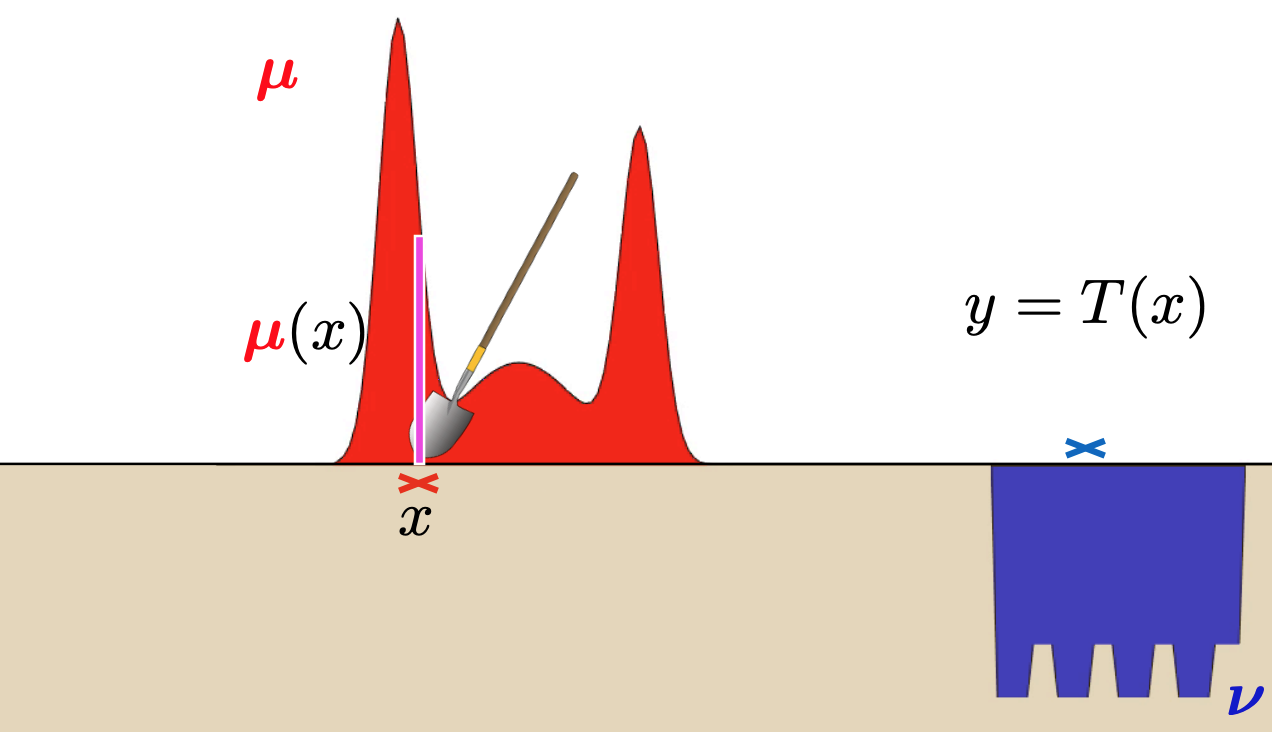
\includegraphics[width=\linewidth]{Figures/EMD_shovel.png}
\end{frame}

\begin{frame}\frametitle{Problem: Moving dirt}
This defines a relationship between measures $\mu$ and $\nu$
\bigskip
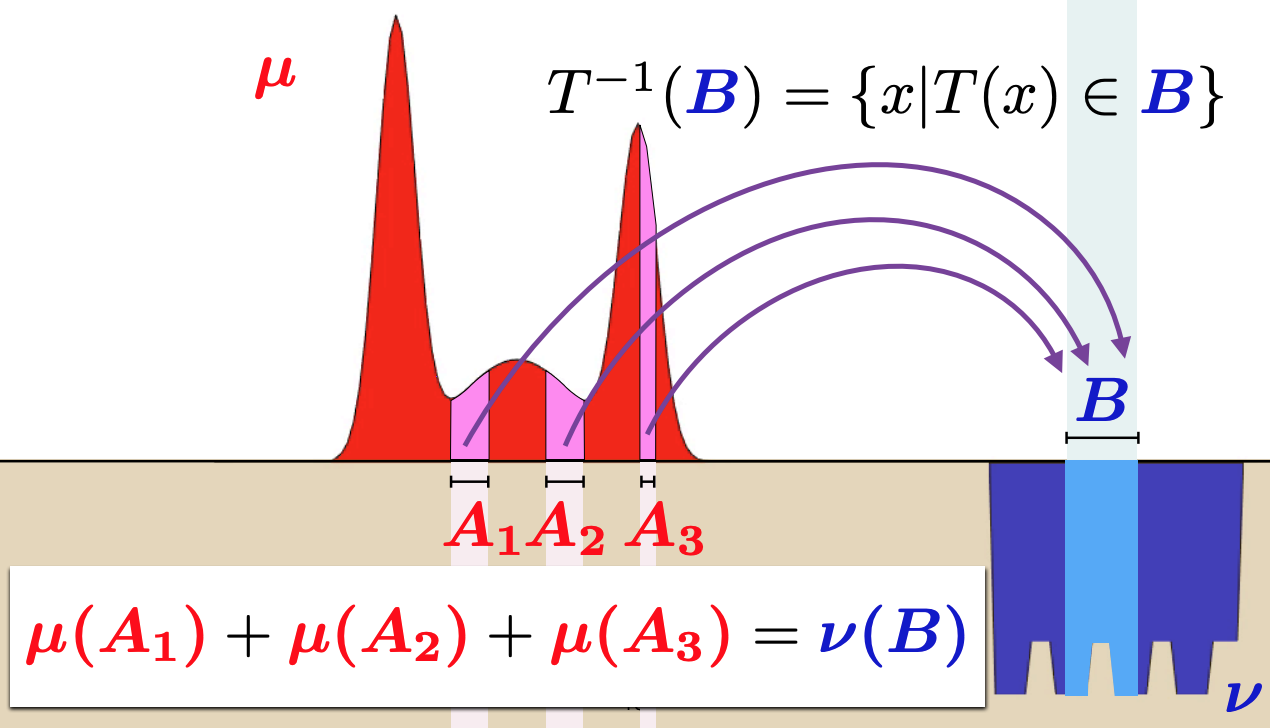
\includegraphics[width=\linewidth]{Figures/EMD_pushforward.png}
\end{frame}

\begin{frame}\frametitle{Pushforward mesaure}
\begin{itemize}
\item
Let $\mathbf T : \mathcal X \to \mathcal Y$ be a continuous map from sample space $\mathcal X$ to sample space $\mathcal Y$.
\item
The pushforward operator $\mathbf T_\sharp : \mathcal M(\mathcal X) \to \mathcal M(\mathcal Y)$, which maps measures on $\mathcal X$ to measures on $\mathcal Y$, satisfies for a given measure $\mu \in \mathcal M(\mathcal X)$,
 $\forall B \subset \mathcal Y$, $B$ measurable, we have
\begin{align}
    \left(\mathbf T_\sharp \mu\right) (B) 
    & = \mu\left( \{ \mathbf x \in \mathcal X : \mathbf T(\mathcal X) \in B \} \right) \\
    & = \mu\left(\mathbf T^{-1}(B) \right)
\end{align}

In the discrete case, which will be the case for TCR repertoires, we have
\ba
    \mathbf T_\sharp \mu := \sum_{i=1}^n a_i \delta_{\mathbf T(\mathbf x_i)}
\ea
for some weights $a_1, \dotsc, a_n$. 
\end{itemize}
\end{frame}

\begin{frame}\frametitle{}
\begin{itemize}
\item
Let $\mu(\bx) D(\bx, \bT(\bx))$ be the work to move the mass at $\bx$ to $\bT(\bx)$
\item
We seek the $\bT$ which minimizes the total work over our domain $\mathcal X$:
\ba
\estim \bT 
	& = \argmin_{\bT_\sharp\mu = \nu} \int_{\mathcal X} D(\bx, \bT(\bx)) \;\der \mu(\bx)
\ea
\item
This is known as Monge's problem
\item
This is a strict formulation and cannot be applied to most practical problems
\item
But, it's easy to picture and sets up the intuition for more general problems
\end{itemize}
\end{frame}

\begin{frame}\frametitle{Moving books: the importance of the cost function}
Suppose that we have n books of equal width on a shelf (the real line), arranged in a single contiguous block. We wish to rearrange them into another contiguous block, but shifted one book-width to the right. Two obvious candidates for the optimal transport plan present themselves:
\begin{itemize}
\item
move all n books one book-width to the right ("many small moves")
\item
move the left-most book n book-widths to the right and leave all other books fixed ("one big move").
\end{itemize}
If the cost function is proportional to Euclidean distance ($c(x, y) = \alpha|x - y|$) then these two candidates are both optimal. If, on the other hand, we choose the strictly convex cost function proportional to the square of Euclidean distance ($c(x, y) = \alpha|x - y|^2$), then the "many small moves" option becomes the unique minimizer.
\end{frame}

\begin{frame}\frametitle{Justification for entropic regularization}
Basic rationale:
\begin{align*}
\; & \text{Entropic constraint} \\
& \implies \text{principile of maximum entropy} \\
& \implies \text{most smooth joint probability given a cost level} \\
& \implies \text{more robust notion of distance}
\end{align*}
For a given pair $({\color{red} \mathbf r}, {\color{blue} \mathbf c})$, finding plausible transportation plans with low cost (where plausibility
is measured by entropy) is more informative than finding extreme plans that are
extremely unlikely to appear in nature
\end{frame}

\begin{frame}\frametitle{Visualizing entropic regularization}
\begin{center}
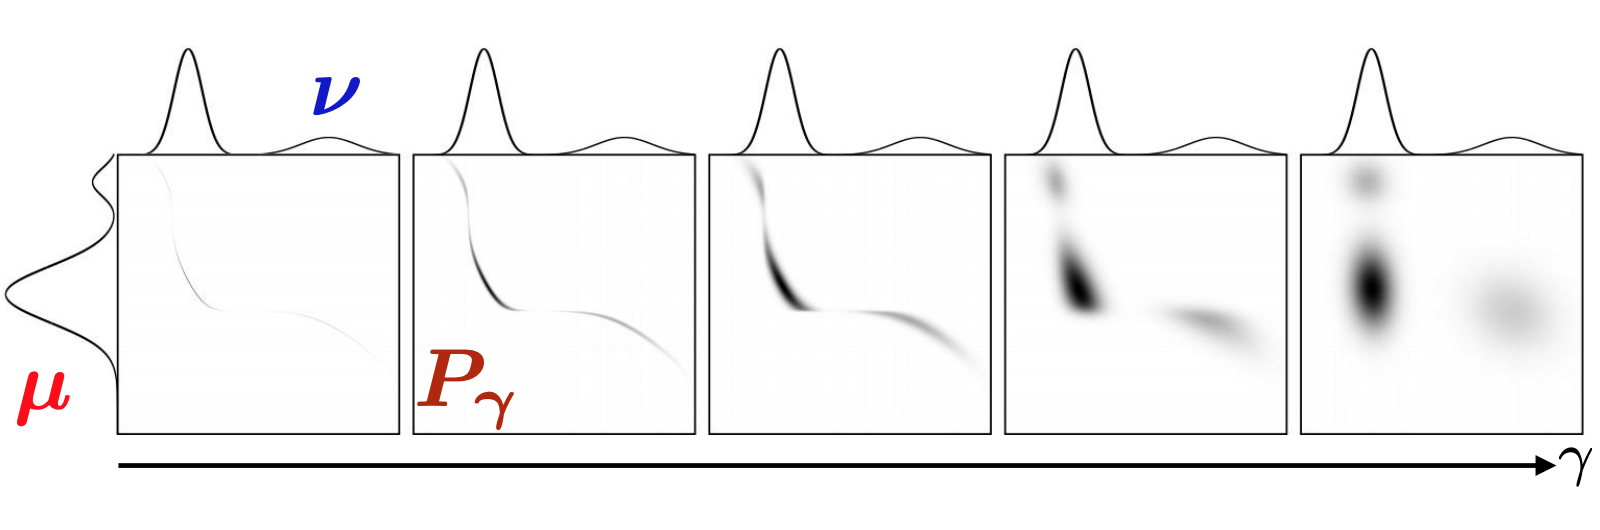
\includegraphics[width=\linewidth]{Figures/EntropyPlots.png}
\end{center}
* Here, $\gamma := \frac{1}{\lambda}$
\end{frame}

\begin{frame}\frametitle{Bernoulli couplings}
\begin{center}
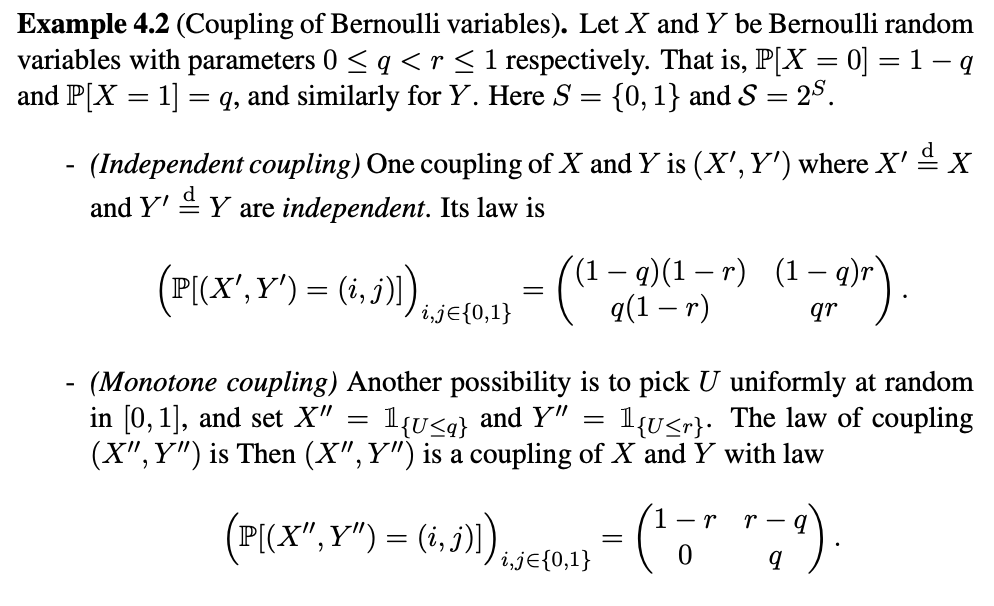
\includegraphics[width=\linewidth]{Figures/Bernoulli.png}
\end{center}

\end{frame}

\end{document}























